\documentclass[14pt]{beamer}

\usepackage[T2A]{fontenc}
\usepackage{fontspec}
\usepackage[utf8]{inputenc}
\usepackage[english,russian]{babel}

\setmainfont[Mapping=tex-text]{CMU Serif}
\setsansfont{CMU Sans Serif}
% \setmonofont{CMU Typewriter Text}


\usepackage{amssymb,amsfonts,amsmath,mathtext}
\usepackage{bussproofs}
\usepackage{stmaryrd}
\usepackage{anyfontsize}

\usepackage{enumerate,float,indentfirst}

\usepackage[
backend=biber,
style=alphabetic,
sorting=ynt
]{biblatex}
\addbibresource{presentation.bib}

\graphicspath{{images/}}

\usetheme{Pittsburgh}
\usecolortheme{whale}

\setbeamercolor{footline}{fg=blue}
\setbeamertemplate{footline}{
  \leavevmode%
  \hbox{%
  \begin{beamercolorbox}[wd=.333333\paperwidth,ht=2.25ex,dp=1ex,center]{}%
    Шамиль Гарифуллин, СПбАУ
  \end{beamercolorbox}%
  \begin{beamercolorbox}[wd=.333333\paperwidth,ht=2.25ex,dp=1ex,center]{}%
    СПбАУ, 2016
  \end{beamercolorbox}%
  \begin{beamercolorbox}[wd=.333333\paperwidth,ht=2.25ex,dp=1ex,right]{}%
  Стр. \insertframenumber{} из \inserttotalframenumber \hspace*{2ex}
  \end{beamercolorbox}}%
  \vskip0pt%
}

\newcommand{\itemi}{\item[\checkmark]}

\title{\small{Генерация зависимых языков по спецификации пользователя}}
\author{\small{%
\emph{Выступающий:}~Шамиль Гарифуллин\\%
\emph{Руководитель:}~Валерий Исаев}\\%
\vspace{30pt}%
Санкт-Петербургский Академический Университет%
\vspace{20pt}%
}
\date{\small{СПбАУ, 2017}}

\begin{document}

\maketitle

\begin{frame}
\frametitle{Соответствие Карри-Говарда}
Описаны в \cite{palmgren2007partial, isaev2016algebraic}\\

\emph{Сигнатура} -- пара $(\mathcal{S},\mathcal{F})$,
    $\mathcal{S}$ -- произвольное множество, $\mathcal{F}$ -- множество и функция,
    которая каждому $f \in \mathcal{F}$ сопоставляет его тип

\begin{center}
\AxiomC{}
\RightLabel{, $x \in Var$, $x : s$}
\UnaryInfC{$x : s$}
\DisplayProof
\end{center}

\begin{center}
\AxiomC{$t_1 : s_1$}
\AxiomC{\ldots}
\AxiomC{$t_n : s_n$}
\RightLabel{, $f : s_1 \times \ldots \times s_n \to s$}
\TrinaryInfC{$f(t_1, \ldots t_n) : s$}
\DisplayProof
\end{center}

\end{frame}


\begin{frame}
\frametitle{Пример определения языка - теории в тт}
\emph{Формула} в сигнатуре $\Sigma$ -- это выражение вида $t = t'$, где $t$ и $t'$ -- термы сигнатуры $\Sigma$ одного сорта.

\begin{figure}[H]
  \center
  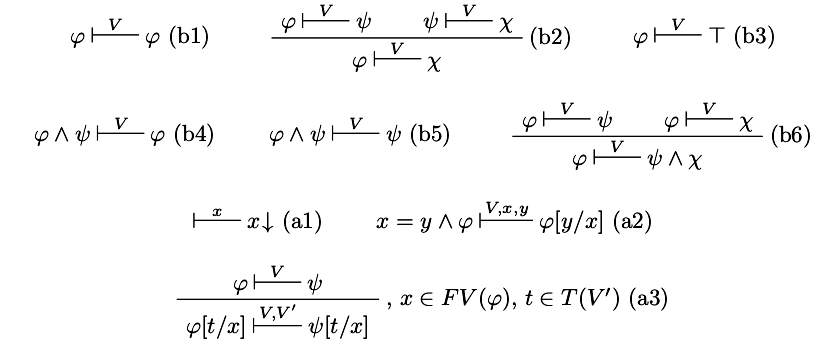
\includegraphics[width=1.0\linewidth]{vlai}
\end{figure}
\end{frame}


\begin{frame}
\frametitle{Зависимые языки - веселый пример из тт}
\emph{Формула} в сигнатуре $\Sigma$ -- это выражение вида $t = t'$, где $t$ и $t'$ -- термы сигнатуры $\Sigma$ одного сорта.

\begin{figure}[H]
  \center
  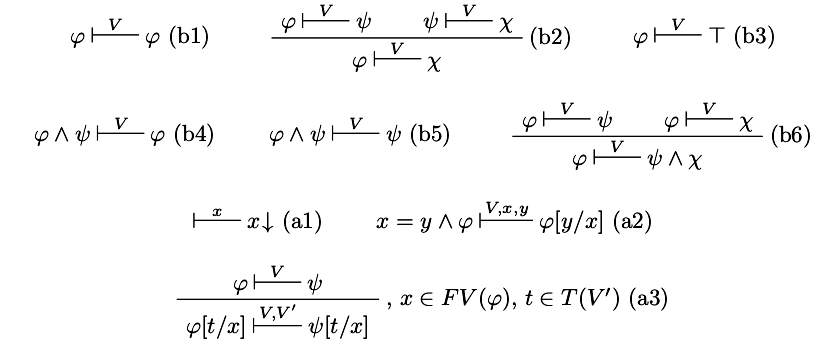
\includegraphics[width=1.0\linewidth]{vlai}
\end{figure}
\end{frame}

\begin{frame}
\frametitle{Цели и задачи}
\begin{itemize} %[<+->]
  \item Создать язык для генерации проверки типов в зависимых языках
  \item Сделать его удобным для использования
  \begin{itemize}
    \item Вывод ошибок пользователя при написании доказательств
    \item Простота добавления новых конструкций
    \item Автоматизация частей доказательств
  \end{itemize}
  \item Написать пример работы для ознакомления с использованием EDSL
\end{itemize}
\end{frame}

\begin{frame}
\frametitle{Вот пример спецификации языка}
\begin{itemize} %[<+->]
  \item Проверка типов термов, формул и секвенций
  \item Вывод ошибок пользователя на уровне типов
  \item typeclass для $(\mathcal{S},\mathcal{F})$ и для аксиом пользователя
  \item Проверка доказательств с выводом ошибок применения правил
\end{itemize}
\end{frame}

\begin{frame}
\frametitle{Проверка нашего языка?}
\begin{itemize} %[<+->]
  \item Неудобство использования правил
  \begin{itemize}
    \item Неудобны для применения на концептуальном уровне
    \item Невозможность расширять пользовательскими правилами
  \end{itemize}
  \item Вывод термов и доказательств на экран
  \item $t(x, y) :== f(g(x,f(x,y)), g(y,x))$
\end{itemize}
\end{frame}

\begin{frame}
\frametitle{Генерация языка - смотрим и все рекурсивно определено}
\begin{figure}[H]
  \center
  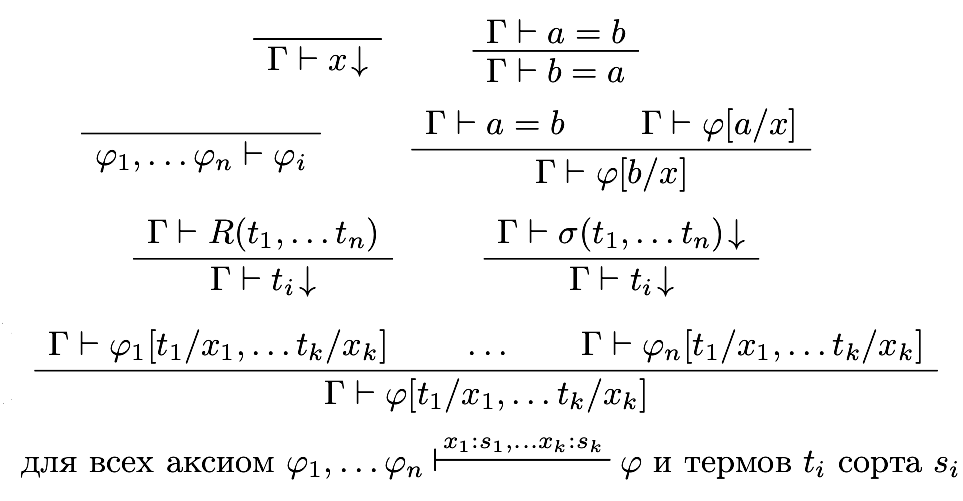
\includegraphics[width=1.0\linewidth]{vlai2}
\end{figure}
\end{frame}


\begin{frame}
\frametitle{Индексы де брейна - опиши проблемы подстановки и альфа равенства, опиши классность на уровне типов, опиши контексты}
\begin{itemize} %[<+->]
  \item Реализованы новые правила вывода
  \item Возможность добавлять пользовательские правила \cite{swierstra2008data, bahr2014composing}
  \item type MyProof = (Rule :+: Trans :+: AxiomRule) Axioms Sort Fun
  \item Общий Pretty Printing расширяемый пользователем
\end{itemize}
\end{frame}

\begin{frame}
\frametitle{Результаты}
\begin{itemize}
  \item Высокоуровневый язык спецификации языков прогрмаммирования с зависимыми типами
  \item Генерация модуля с фукциями проверки типов и приведения в нормальную форму
  \begin{itemize}
    \item Индексы де Брейна на уровне типов данных
    \item Проверка типов через нормализацию
  \end{itemize}
  \item Примеры спецификации языка
  \item ссыль на репо!
\end{itemize}
\end{frame}

\begin{frame}
\frametitle{Дальнейшее работа??}
\begin{itemize}
  \item Проверка программ - отличие в функциях и парсере
\end{itemize}
\end{frame}

\begin{frame}[shrink=20]
\frametitle{Список литературы}
\printbibliography
\end{frame}


\end{document}
